\documentclass[a4paper,12pt]{article}%\documentclass[a4paper,12pt,titlepage]{article}

%\usepackage{palatino}
\usepackage{graphicx}
\usepackage{epstopdf}
\usepackage{epsfig}
\usepackage{listings}
\usepackage{color}
\usepackage{subfigure}
\usepackage{enumerate}
\usepackage{url}
%數學公式
\usepackage{amsthm,amsfonts}
\usepackage{amsmath,bm}              % AMSLaTeX
\usepackage{amssymb,mathrsfs}        % AMSLaTeX sym-bols
\usepackage{latexsym}
\usepackage[UTF8]{ctex}

% style: list typesetting
\definecolor{grey}{rgb}{0.8,0.8,0.8}
\definecolor{darkgreen}{rgb}{0,0.3,0}
\definecolor{darkblue}{rgb}{0,0,0.3}
\def\lstbasicfont{\fontfamily{pcr}\selectfont\footnotesize}
\lstset{%
% indexingh
   % numbers=left,
   % numberstyle=\small,%
% character display
    showstringspaces=false,
    showspaces=false,%
    tabsize=4,%
% style
    frame=lines,%
    basicstyle={\footnotesize\lstbasicfont},%
    keywordstyle=\color{darkblue}\bfseries,%
    identifierstyle=,%
    commentstyle=\color{darkgreen},%\itshape,%
    stringstyle=\color{black}%
    }
\lstloadlanguages{C,C++,Java,Matlab,Mathematica}
\graphicspath{{./}{./img/}{./fig/}{./image/}{./figure/}{./picture/}}
% style: page layout
\setlength{\headheight}{15pt}
\setlength{\headsep}{20pt}
\setlength{\footskip}{30pt}
\setlength{\voffset}{-5pt}
\setlength{\hoffset}{16pt}
\setlength{\oddsidemargin}{0pt}
\setlength{\evensidemargin}{\oddsidemargin}
\setlength{\marginparpush}{0pt}
\setlength{\marginparwidth}{0pt}
\addtolength{\textheight}{3\baselineskip}


%%%%%%%%%%%%%%%%%%%%%%%%%%%%%%%%%%%%%%%%%%%%%%%%%%%%%%%%%%%%%%%%%%%
%%%%%%%%%%%%%%%%%%$$$$$$$==濞e繑浜濈紘鎻掔暜==$$$$$$$%%%%%%%%%%%%%%%%%%%%%%%
%%%%%%%%%%%%%%%%%%%%%%%%%%%%%%%%%%%%%%%%%%%%%%%%%%%%%%%%%%%%%%%%%%%

%==========================闊附浜濆鎾寸亞===============================
\title{Digital Imaging Processing\\ 數字影像處理 \\ Project Three  }
\author{\small Lin Dongwen}
\date{05, 2013}
%=================================================================
%==================================================================
\begin{document}
    \maketitle
    \newpage
%\section{Background}
%Reversible data embedding, which is also called lossless data embedding,
%embeds invisible data (which is called a payload or a watermark) into a digital image
% called "cover image" in a reversible fashion. The performance of a reversible data-embedding a
% lgorithm can be measured by the following:
%
%%Reversible data embedding又叫 lossless data embedding, 是把invisible data(一般又叫payload或watermark)植入一個數字影像(cover image)的一種方法。其優劣性主要通過下面的指標來衡量
%\begin{center}
%\begin{description}
%    \setlength{\itemsep}{0pt}
%    \setlength{\parskip}{0pt}
%    \setlength{\parsep}{0pt}
%    \item[Complexity] The algorithm complexity.% 算法複雜度
%    \item[Visual quality] Visual quality. % 影像質量
%    \item[Payload capacity limit] Maximal amount of information can be embedded. % 最大可植入的數據量
%\end{description}
%\end{center}

\section{Step 1:Haar Wavelet transform}
\subsection{Background Knowledge——背景知識}

\noindent 首先看維基百科里關於Wavelet Transform的相關簡介:
\begin{quote}

The Haar transform is the simplest of the wavelet transforms. This transform cross-multiplies a function against the Haar wavelet with various shifts and stretches, like the Fourier transform cross-multiplies a function against a sine wave with two phases and many stretches.

\textbf{Scaling function.} Wavelets are defined by the wavelet function $\psi(t)$ (i.e. the mother wavelet) and scaling function $\phi(t)$ (also called father wavelet) in the time domain.

\textbf{Wavelet function.} The wavelet only has a time domain representation as the wavelet function $\psi(t)$.
For instance, Mexican hat wavelets can be defined by a wavelet function.
\end{quote}

\subsection{How to}

From the question we know that scaling function is {1/2,1/2} ,
while the wavelet coefficients function is {1,-1}. Let N be the
length of $X_n$, we will have M = [$\frac{X_n}{2}$], we will have

\begin{equation}
L_k=\frac{1}{2}(x_{2k-1} + x_{2k});
\end{equation}

\begin{equation}
H_k=|(x_{2k-1} - x_{2k}|;
\end{equation}

\subsection{The result}
    The result can be seen in \eqref{fig:subfig:a}

\begin{figure}[h]
  \centering
  \subfigure[Horizontally Produced Lena]{
    \label{fig:subfig:a} %% label for first subfixgure
    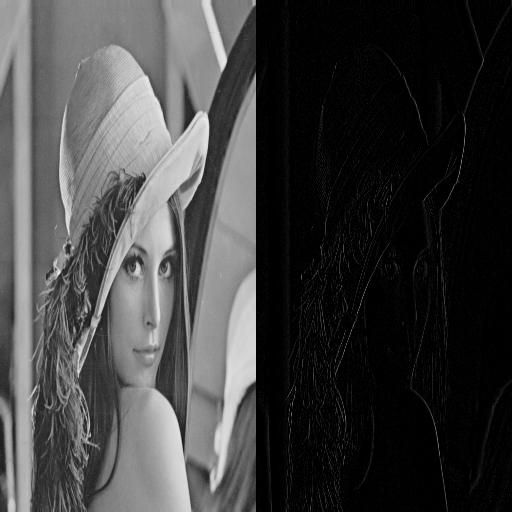
\includegraphics[width=2in]{./figure/horizontally_produce.jpg}}
  \hspace{0.5in}
  \subfigure[Verticallly Produced Lena]{
    \label{fig:subfig:b} %% label for second subfigure
    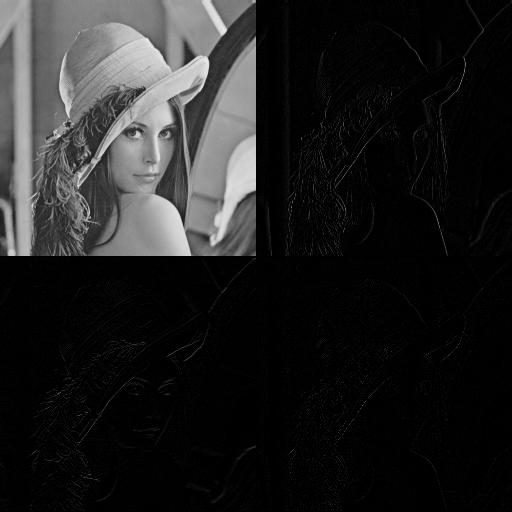
\includegraphics[width=2in]{./figure/vertically_produce.jpg}}
    \hspace{0.5in}
  \caption{The result for the first problem}
  \label{fig:subfig} %% label for entire fig
\end{figure}

Similarly, we can utilize the same method Vertically.See fig\eqref{fig:subfig:b}.

\textbf{The related code is in main.m: Step 1 and Haar Wavelet transform is in hwt.m}

\section{Step 2:Watermark 2 Binary}
\subsection{How to}
    第二步需要做的是把要植入的水印做變化使它變為Binary的Code,圖像在這裡會丟失一些內容。
變為兩個明暗度。然後再對其做行列變化使其變為一列。比如說原來是M行N列的矩陣,在變化后,
變為有$M\times N$個元素的行向量。
\subsection{The result}
    詳細可看附的文件夾中文件名為“Myname.jpg”(變化前)的文件,和文件名為“bits.jpg”(變化后)
的文件。分別是做變化前的水印和變化后的水印。相關代碼參見main.m的Step 2的部份。

\section{Step 3:Embeding}
第三步要做的是Watermark的Embed的過程。這一步是整個程式里最核心的部份。

\subsection{Related Knowledge}
加密算法主要通過Haar Wavelet Transform來實現,也叫做Interger Wavelet Transform或Difference Expansion Transform,The difference Expansion的原理如下:

假設需要展開兩個值$x = 206$, $y = 201$, 則有
$$
l = [\frac{206+201}{2}]=[\frac{407}{2}],h = 206 - 201 = 5
$$
我們想要在裏面植入bit=1的話,讓
$$h' = 2 \times h + b = 2 \times 5 + 1$$
這樣新的值就變成了
$$x = l + [\frac{h+1}{2}] = 209, y = l - [\frac{h}{2}]=198$$

通過這樣的原理就可以植入bit在圖像裏面。

爲了區別植入和沒有植入的變量,我們又新引入了一個闕值T。根據T將圖像中的點分成不同的情況:

\begin{itemize}
  \item 如果 $|h| \leq [\frac{T}{2}]$ 則為集合 M
  \item 如果 $ 2T + 1 \geq |h| > [\frac{T}{2}] $ 則為集合 N
  \begin{itemize}
    \item 如果 $ T \geq |h| > [\frac{T}{2}] $則為集合 $N_e$
    \item 如果 $ 2T + 1 \geq |h| > T  $則為集合 $N_{\bar{e}}$
  \end{itemize}
  \item 如果 $|h| > 2T + 1$ 則為集合 U
\end{itemize}

藏數據的時候,我們會把所有的數據都藏在集合$N_{e}$和$M$裏面。

\textbf{關於T值確定的辦法:}

    在Decode的時候,由於集合$N_e$和$N_{\bar{e}}$的確定需要Map才能確定,這樣才能保證能夠恢復到原圖片。而在N裏面只有$N_e$是可以藏數據的,所以一共只能藏$M - N_{\bar{e}}$個的數據,首先確定需要藏的水印的大小,然後根據這個大小來確定需要T的最小值。T越大,則圖像的失真會越大。具體的確定算法參見\textbf{caculate\_T.m}

\subsection{How to}

\begin{description}
\setlength{\itemsep}{0pt}
\setlength{\parskip}{0pt}
\setlength{\parsep}{0pt}
      \item[Step0]首先計算T的值得大小。
      \item[Step1]通過引入一個同圖像像素行列相同的矩陣ID來表示圖像每一個屬於的集合類型
      \item[Step2]根據矩陣ID來得出Map表,用來表示矩陣$N_e$和$N_{\bar{e}}$
      \item[Step3]將Map與Payload連接起來,然後首先把數據藏在$M$矩陣之中,然後再把
剩下的數據藏在$N_e$里。加密的時候利用加密算法。%Step 3.Watermark_Embeding
\end{description}

\subsection{The result}
    The result can be seen in fig \eqref{fig:marked}

\begin{figure}
  \centering
  % Requires \usepackage{graphicx}
  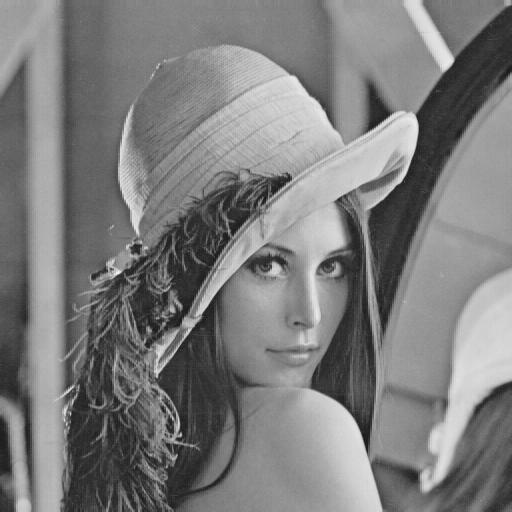
\includegraphics[width=5in]{./figure/marked.jpg}\\
  \caption{watermarked}\label{fig:marked}
\end{figure}

\section{Step 4:Compute the Histogram}
    \subsection{Related Knowledge}
        在計算機圖像學領域中,常用一種灰度直方圖。灰度直方圖是灰度級的函數,描述的是圖像中具有該灰度級的像素的個數:橫坐標是灰度級,縱坐標是該灰度出現的頻率(像素個數)。
    \subsection{How to}
        使用Matlab的一個函數叫imhist即可繪出直方圖(需要注意的是先把圖片換成uint8的類型)
    \subsection{The result}
        The result can be seen in fig

\begin{figure}
  \subfigure[Horizontally Produced Lena]{
    \label{fig:subfig:a} %% label for first subfixgure
    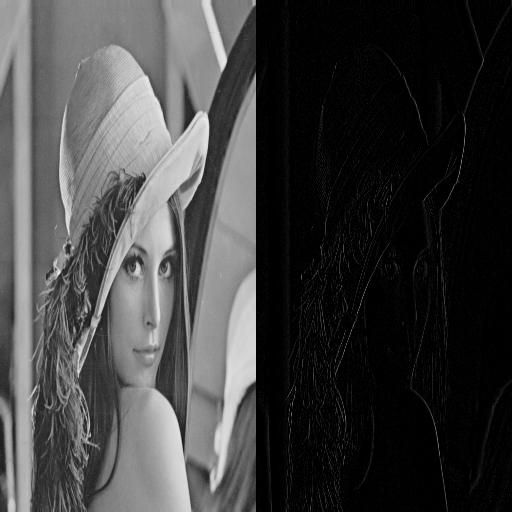
\includegraphics[width=3in]{./figure/horizontally_produce.jpg}}
  \hspace{2in}
  \subfigure[Verticallly Produced Lena]{
    \label{fig:subfig:b} %% label for second subfigure
    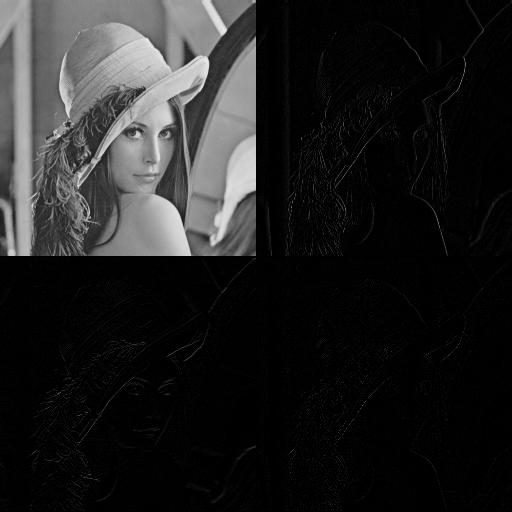
\includegraphics[width=3in]{./figure/vertically_produce.jpg}}
    \hspace{2in}
  \caption{The result for the first problem}
  \label{fig:subfig} %% label for entire fig
\end{figure}

\section{Step 5:Decoding}
    \subsection{How to}
Decoding的過程與encoding的過程恰好相反,可以將水印從圖片里提取出來,同時也會將圖像還原到原來的情況。

Decoding的相關算法如下:
\begin{description}
      \item[Step1]根據T的值與H的值把不同的點對按照集合劃分為三類,M,N和U,分別標記其ID,$ID=1$為U
$ID=4$為M,$ID=5$為N。
      \item[Step2]根據N的大小計算出Map的位數,并從M中取出Map。
      \item[Step3]依據Map把N分為$N_e$和$N_{\bar{e}}$。標記ID,
$ID=2$為$N_{\bar{e}}$,$ID=3$為$N_e$,
      \item[Step4]根據ID對$M$($ID=4$,先恢復)以及$N_e$($ID=3$,后恢復)進行復原,並提取出Bit。
\end{description}
\subsection{The result}
The result can be seen in fig
\begin{figure}
  \centering
  % Requires \usepackage{graphicx}
  
\includegraphics[width=5in]{./figure/myname.JPG}\\
  \caption{watermarked}\label{fig:marked}
\end{figure}


\begin{figure}[h]
  \centering
  \subfigure[The water mark]{
    \label{fig:subfig:a} %% label for first subfixgure
      
\includegraphics[width=2in]{./figure/myname.JPG}}
  \hspace{0.5in}
  \subfigure[Verticallly Produced Lena]{
    \label{fig:subfig:b} %% label for second subfigure
    
\includegraphics[width=2in]{./figure/d_watermark.jpg}}
    \hspace{0.5in}
  \caption{See the watermark original one and the decoding one}  \label{fig:subfig} %% label for entire fig
\end{figure}

\begin{figure}
\centering
  % Requires \usepackage{graphicx}
  \caption{The Water Mark}\label{fig:watermark}
\end{figure}


\section{Step 6:Compare the extracted binary signature and the recovered image}
    \subsection{How to}
	使用Matlab的函數imhist繪出直方圖即可,同理需要先把圖像變換成uint8的類型
    \subsection{The result}
	The result can be seen here.

\section{Source Code}

Here are the source code for this project.\\

\textbf{\textcolor[rgb]{0.98,0.00,0.00}{Input matlab source:}}
\lstinputlisting[language=Matlab]{../main.m}

\textbf{\textcolor[rgb]{0.98,0.00,0.00}{Input matlab source:}}
\lstinputlisting[language=Matlab]{../lib/hwt.m}

\textbf{\textcolor[rgb]{0.98,0.00,0.00}{Input matlab source:}}
\lstinputlisting[language=Matlab]{../lib/myimshow.m}

\textbf{\textcolor[rgb]{0.98,0.00,0.00}{Input matlab source:}}
\lstinputlisting[language=Matlab]{../lib/caculate_T.m}

\begin{thebibliography}{99}
\addcontentsline{toc}{section}{References}
\bibitem{1} Jun Tian, Reversible Data Embedding Using a Difference Expansion, IEEE, 2003
\bibitem{2} wikipedia.\url{http://en.wikipedia.org/wiki/Haar_wavelet}
\end{thebibliography}

\end{document}